\documentclass[UTF8,fontset=none,12pt]{ctexart}

\setCJKmainfont{Songti SC}
\setCJKsansfont{PingFang SC}
\setCJKmonofont{Songti SC}

\usepackage[a4paper,margin=2.35cm]{geometry}
\usepackage{amsmath,amssymb,amsthm,mathtools,bm}
\usepackage{graphicx}
\usepackage{float}
\usepackage{booktabs}
\usepackage{array}
\usepackage{enumitem}
\usepackage[hidelinks]{hyperref}

\title{数值线性代数\quad 第 32 讲：迭代法概述}
\author{Lloyd N. Trefethen、David Bau III\quad 中文阅读版}
\date{}

\begin{document}
\maketitle
\pagestyle{plain}

从本讲开始，本书的风格发生变化。我们将从已经相当成熟的经典主题——直接法，
转向相对而言仍然充满未知的迭代法领域。迭代法很可能主导未来的大规模计算。

\section*{为什么要迭代？}

线性代数中迭代算法的重要性源于一个简单事实：非迭代的“直接”算法通常需要
$O(m^3)$ 的运算量。这太多了！一方面，当 $m$ 很大时，$m^3$ 的绝对数值本身
就非常大；另一方面，大多数矩阵问题的输入只包含 $O(m^2)$ 个数，因此解决问题
却必须花费 $O(m^3)$ 次运算，似乎也不合理。

下面的表格给出了多年来矩阵计算规模的大致历史：

\begin{center}
\begin{tabular}{rcl}
1950: & $m=20$ &（Wilkinson）\\
1965: & $m=200$ &（Forsythe 和 Moler）\\
1980: & $m=2000$ &（UNPACK）\\
1995: & $m=20000$ &（LAPACK）
\end{tabular}
\end{center}

这些数字粗略表示，在相应年代，人们可能认为“非常大”的稠密直接矩阵计算问题
的维数。在 20 世纪 60 年代中期的“Forsythe 和 Moler 时代”（名称来自一本
1967 年出版的有影响力的教材）中，几百维的矩阵就已经很大，几乎达到当时机器
能够在合理时间内处理的极限。

显然，在 45 年间，可处理矩阵问题的维数增加了 $10^3$ 倍。这一进步令人印象
深刻，但与同一时期计算机硬件从每秒浮点运算到每秒十亿次浮点运算所带来的
$10^9$ 倍加速相比，仍然相形见绌。由于 $10^9$ 正好是 $(10^3)^3$，历史上
已经清楚地展现了直接矩阵算法的 $O(m^3)$ 瓶颈。

换一种说法：如果矩阵问题能够用 $O(m^2)$ 而不是 $O(m^3)$ 次运算解决，那么
今天处理的一些矩阵的规模或许还能扩大 10 到 100 倍。这正是矩阵迭代法所追求
的目标——对某些矩阵已经实现，对另一些矩阵则未必能够实现。

\section*{结构、稀疏性与黑盒}

当然，$O(m^3)$ 瓶颈并不显然能够被突破；对于“随机”的矩阵问题，答案很可能
是否定的。然而，实际出现的大型矩阵远非随机，原因很简单。小矩阵（比如 3 维
或 30 维）可能在科学问题中直接产生，条目近似任意，例如表示结构中三个力之间
的关系，或化学反应中三十种物质之间的关系。相比之下，大矩阵通常间接产生于
微分方程或积分方程的离散化。可以说，如果 $m$ 非常大，它很可能是在逼近无穷
维问题。

因此，大多数具有计算意义的大矩阵虽然含有数量庞大的条目，但结构往往比表面
上看起来简单得多。它们具有某种结构；随着时间推移，人们也在越来越多的场景
中找到了利用这些结构的方法。

大型矩阵最明显的结构是稀疏性，即零条目占绝大多数（稀疏的反义词是稠密）。
例如，偏微分方程的有限差分离散可能产生一个维数为 $m=10^5$ 的矩阵，每行只有
$\nu=10$ 个非零条目。这种结构很容易被本书后面讨论的迭代法利用，因为这些
算法把矩阵当作一个黑盒：

\begin{figure}[H]
\centering
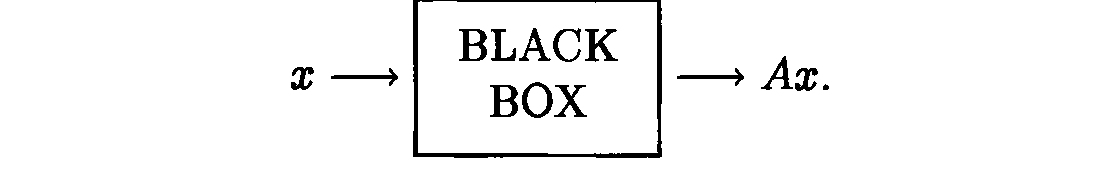
\includegraphics[width=0.58\textwidth]{../assets/figure-32-black-box.png}
\parbox{0.58\textwidth}{\small 黑盒只需接收任意向量 $x$，并返回矩阵--向量积 $Ax$。}
\end{figure}

迭代算法只要求能够对任意 $x$ 确定 $Ax$。在计算机程序中，这由一个过程完成，
而该过程的内部实现不需要由迭代算法的设计者了解。（某些迭代算法还需要计算
$A^*x$。）对于稀疏矩阵 $A$，很容易设计一个过程，用仅 $O(\nu m)$ 而不是
$O(m^2)$ 次运算计算 $Ax$。这与直接线性代数算法形成鲜明对比：高斯消去法或
Householder 三角化会显式操作矩阵条目以引入零，但在这一过程中通常又会破坏
稀疏性。

从历史上看，稀疏性是迭代矩阵计算中最常被利用的结构。（嵌套剖分、最小度重
排序等快速直接法也利用稀疏性，但本书不讨论。）近来人们逐渐认识到，即使矩阵
是稠密的，其他类型的结构也可能被利用。例如，用数值方法求解积分方程通常会
得到稠密矩阵问题；工程中称之为边界元法或面元法。这些矩阵的系数往往具有很强
的规律性，因此如何利用这种规律——例如采用多极展开或小波展开——仍是活跃的
研究方向。实现这类方法的黑盒可能包含数千行代码，其背后的思想也只有专家才
能完全理解。

\section*{投影到 Krylov 子空间}

本书余下部分的迭代法都建立在这样一个思想上：把一个 $m$ 维问题投影到一个
低维 Krylov 子空间中。给定矩阵 $A$ 和向量 $b$，相应的 Krylov 序列是

$$
b,\ Ab,\ A^2b,\ A^3b,\ldots,
$$

这些向量可以通过黑盒按如下方式计算：

$$
b,\ Ab,\ A(Ab),\ A(A(Ab)),\ldots.
$$

相应的 Krylov 子空间就是由这些向量中逐渐增大的向量组张成的空间。

具体来说，本书将讨论的算法可以排列成下表：

\begin{figure}[H]
\centering
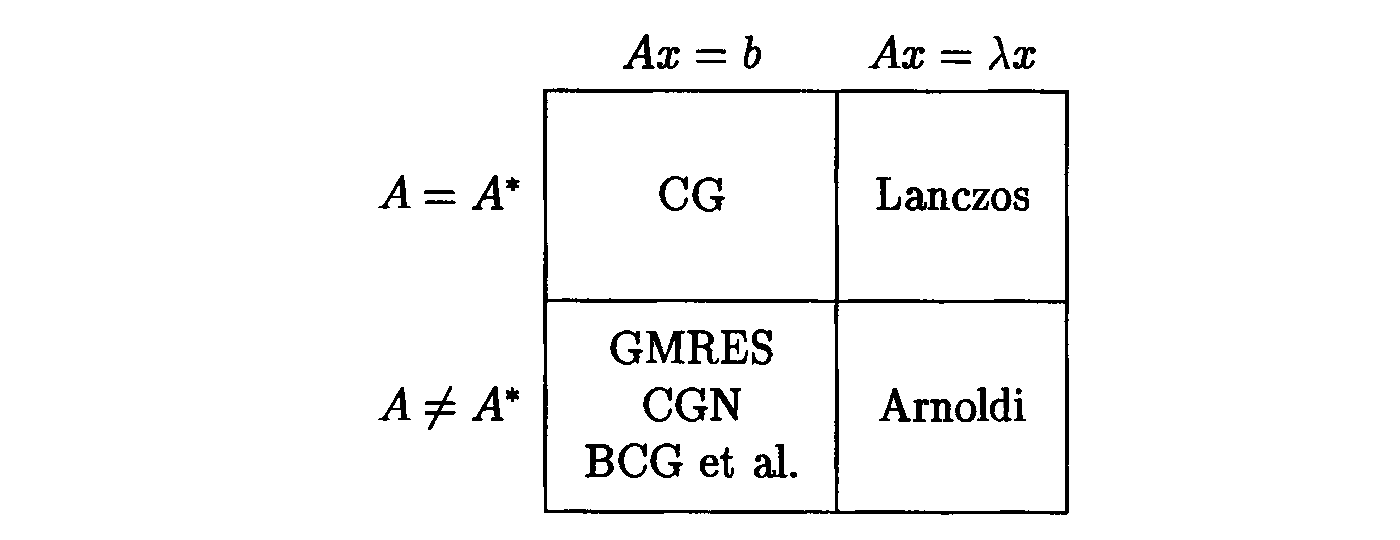
\includegraphics[width=0.76\textwidth]{../assets/figure-32-krylov-table.png}
\parbox{0.76\textwidth}{\small Krylov 投影方法的分类：列区分线性方程组 $Ax=b$ 与特征值问题 $Ax=\lambda x$，行区分 Hermitian 情形 $A=A^*$ 与非 Hermitian 情形 $A\ne A^*$。}
\end{figure}

（这个领域充满了缩写！例如，CG 表示共轭梯度法；顺便说一句，它不仅要求
$A$ 为 Hermitian，还要求 $A$ 正定。）在每一种方法中，投影到 Krylov 子空间
都会把原始矩阵问题约化成一系列维数为 $n=1,2,3,\ldots$ 的矩阵问题。当 $A$
为 Hermitian 时，约化矩阵是三对角的；当 $A$ 非 Hermitian 时，约化矩阵具有
Hessenberg 形式。

例如，Arnoldi 迭代通过计算一系列维数递增的 Hessenberg 矩阵的特征值，来近似
一个大矩阵的特征值。

\section*{步数、每步运算量与预条件}

高斯消去法、QR 分解和稠密线性代数中的大多数其他算法，都符合下面的模式：
共有 $O(m)$ 步，每步需要 $O(m^2)$ 次运算，总运算量估计为 $O(m^3)$。（当然，
在并行计算机上，尤其是第二个数量级可能发生变化。）迭代法也可以用同样的两个
数字描述，但此时它们代表典型的最坏情形。当迭代法成功时，往往能够降低其中
一个或两个因素。

我们将看到，迭代法达到满意精度所需的步数，通常取决于矩阵 $A$ 的谱性质，这里
“谱”应作广义理解。例如，如果 Hermitian 正定系统 $Ax=b$ 的特征值很好地聚集
在远离原点的位置，共轭梯度迭代就能保证快速求解。类似地，如果实 Hermitian
矩阵的某些特征值与其余谱充分分离，并且启动迭代的初始向量足够一般，Lanczos
迭代就能保证快速计算这些特征值。

这些方法的收敛速率分析是一个迷人的研究主题，依赖于逼近论。具体地说，Krylov
子空间迭代算法的收敛性与这样的问题密切相关：在实轴或复平面的某些子集上，
用多项式 $p(z)$ 逼近函数 $f(z)$。

每一步矩阵迭代的运算量，主要取决于矩阵的结构，以及黑盒 $x\mapsto Ax$ 利用
了多少这种结构。

线性代数中理想的迭代法把步数从 $m$ 降到 $O(1)$，把每步运算量从 $O(m^2)$
降到 $O(m)$，从而把总运算量从 $O(m^3)$ 降到 $O(m)$。这种惊人的加速确实会
在实际问题中出现，但更典型的改进也许是把 $O(m^3)$ 降到 $O(m^2)$。

在 20 世纪 90 年代中期的一次大规模工程计算中，对于迭代法能够成功处理的
问题，典型结果或许是比直接法快一个数量级，即大约 10 倍。未来，随着机器变快、
$m$ 变大，这一倍数还会增加，迭代法的重要性也会提高。这体现了计算机科学的一条
基本规律：计算机越快，算法速度的重要性越大。

\section*{精确解与近似解}

从原则上说，矩阵迭代法是近似的：即使没有舍入误差，只要迭代步数停留在实际
感兴趣的范围内，它们也不会给出精确答案。刚接触这些思想的人往往对此感到不安，
可能认为迭代是一种缺乏优雅、可靠性可疑的“工程解法”。但随着对这些方法的
了解加深，这种不安通常会逐渐消失。

毕竟，直接法在计算机上执行时也并不精确：我们希望得到的是机器精度的答案，
而不是比机器精度更高的答案。迭代法同样可以达到机器精度，因此它们在原则上
是近似的这一点并不重要。至于优雅性，本书这里出现的思想是数值线性代数中最
美的一些思想。

这些观点见图 32.1。

\begin{figure}[H]
\centering
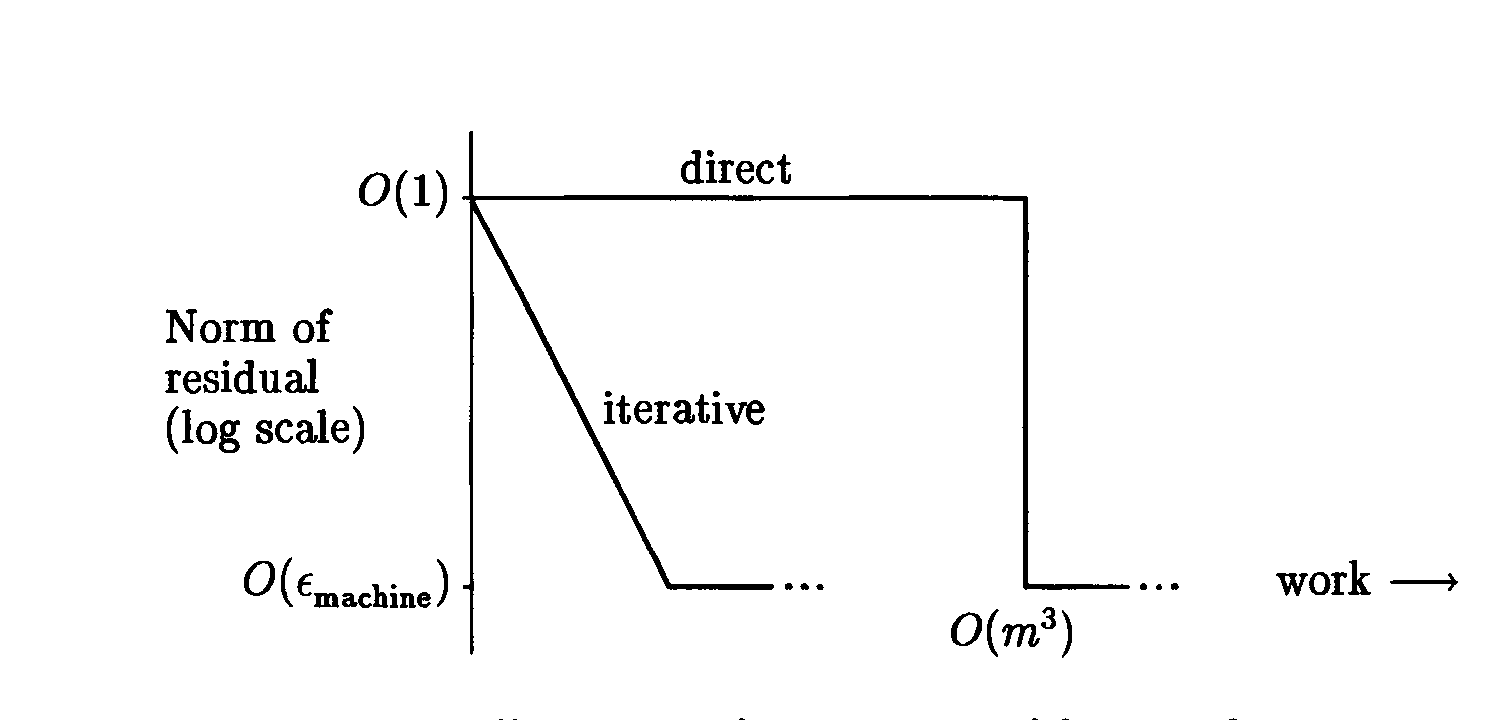
\includegraphics[width=0.90\textwidth]{../assets/figure-32-convergence.png}
\parbox{0.90\textwidth}{\small 图 32.1. 直接法与迭代法收敛过程的示意图。理想情况下，迭代法沿几何速率收敛，直到残差达到 $\varepsilon_{\mathrm{machine}}$ 阶；直接法在完成 $O(m^3)$ 次运算前几乎没有进展，随后残差也达到 $\varepsilon_{\mathrm{machine}}$ 阶。}
\end{figure}

\section*{超越 $O(m^3)$ 的直接法}

最后需要提到，确实存在一些直接算法：它们原则上是有限的、精确的，并且能
以少于 $O(m^3)$ 的运算量求解 $Ax=b$ 及相关问题。

第一种此类算法由 Volker Strassen 于 1969 年发现。他把 Gauss 的指数 3 降到
$\log_2(7)\approx2.81$；随后，Coppersmith 和 Winograd 的改进又把已知最好
指数降到了约 2.376。已知最好指数的历史见图 32.2。

\begin{figure}[H]
\centering
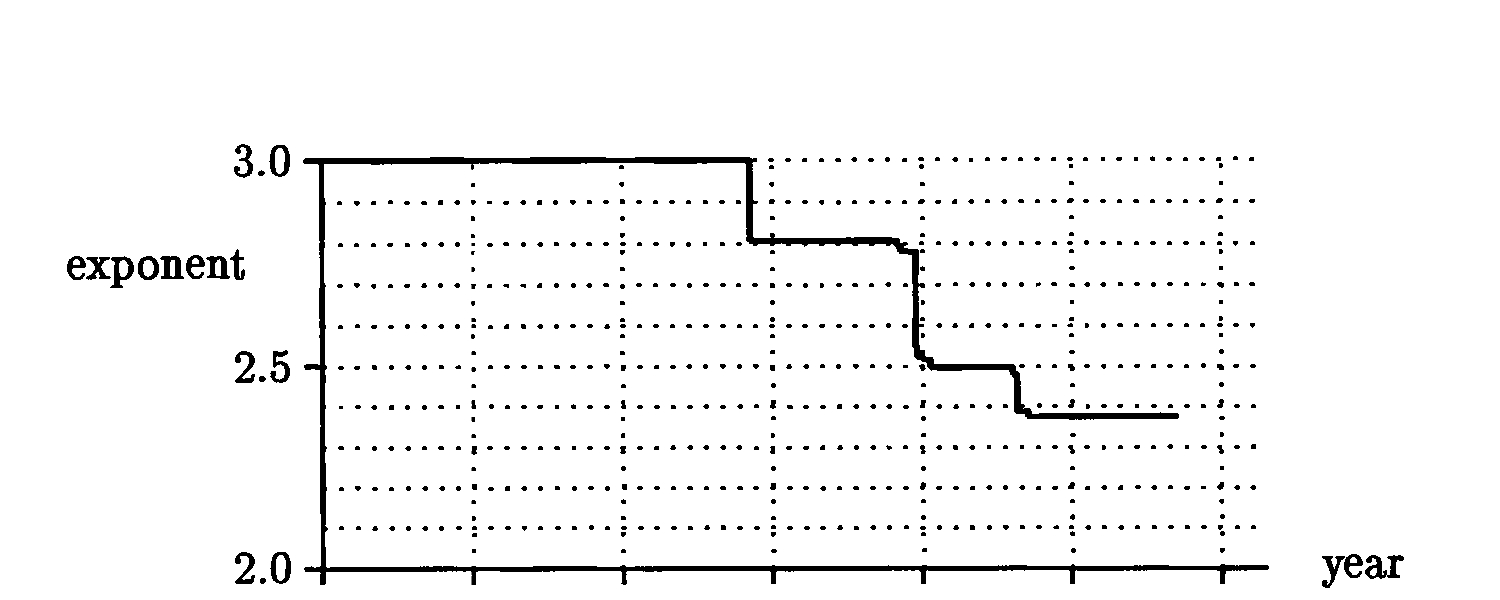
\includegraphics[width=0.90\textwidth]{../assets/figure-32-exponents.png}
\parbox{0.90\textwidth}{\small 图 32.2. $m\times m$ 矩阵直接求解 $Ax=b$（等价地，计算 $A^{-1}$、$AB$ 或 $\det A$）的已知最好复杂度指数随时间的变化。1968 年以前最好算法的复杂度为 $O(m^3)$；目前已知最好算法为 $O(m^{2.376})$，但常数太大，实际上并不实用。}
\end{figure}

到目前为止，这些快速算法对实际计算的影响可以忽略，原因有两个。一个原因
是人们通常并不清楚它们的稳定性性质。更根本的原因是，尽管快速算法的指数
十分引人注目，但它们开始超过标准方法的交叉规模极高。Strassen 的 $m^{2.81}$
算法在 $m$ 低至约 100 时就可能超过高斯消去法；但由于 2.81 离 3 太近，对于
实际规模而言，优势从来不会特别显著。指数远低于这个数的现有方法通常带有很大
的常数因子，因此在当前机器能够达到的规模上仍比高斯消去法慢。

但未来会怎样？没有人知道。

也许明天就有人发现一种“快速矩阵求逆”方法，用
$m^2\log m$ 次浮点运算求解 $Ax=b$；也可能是读者今晚就发现了它。这样的发展
将引发数值计算史上最剧烈的变革。

\section*{习题}

\paragraph{32.1.}
三维椭圆型偏微分方程通过边界元方法离散化。结果是一个大型稠密线性方程组，
其中每个方程对应大球面上的一个三角形面元。为了提高精度，必须把三角形划得
更小，从而增加方程的数量；但误差只会随 $h$ 线性缩小，其中 $h$ 是最大三角形
的直径。

选定一个 $h$ 后，用高斯消去法求解该系统，得到两位有效数字的解，耗时 1 分钟。
现在决定需要三位有效数字。假设存储不是约束，在同一台计算机上重新计算大约需要
多长时间？

\paragraph{32.2.}
考虑分块矩阵乘积

\[
\begin{bmatrix}
W&X\\
Y&Z
\end{bmatrix}
=
\begin{bmatrix}
A&B\\
C&D
\end{bmatrix}
\begin{bmatrix}
E&F\\
G&H
\end{bmatrix},
\]

为简单起见，假设矩阵 $A,B,\ldots,Y,Z$ 都是相同维数的方阵。

\begin{enumerate}[label=(\alph*)]
\item 已知 $A,B,\ldots,G,H$，用直接算法计算 $W,X,Y,Z$ 需要多少次矩阵加法和多少次矩阵乘法？
\item Strassen 证明，也可以用下列公式计算 $W,X,Y,Z$：
\end{enumerate}

\begin{align*}
P_1&=(A+D)(E+H), & P_5&=(A+B)H,\\
P_2&=(C+D)E, & P_6&=(C-A)(E+F),\\
P_3&=A(F-H), & P_7&=(B-D)(G+H),\\
P_4&=D(G-E), &&
\end{align*}

\begin{align*}
W&=P_1+P_4-P_5+P_7, & Y&=P_2+P_4,\\
X&=P_3+P_5, & Z&=P_1+P_3-P_2+P_6.
\end{align*}

现在需要计算：这些公式涉及多少次矩阵加法或减法，以及多少次矩阵乘法？

\begin{enumerate}[label=(\alph*),start=3]
\item 证明：递归地应用 Strassen 公式，可以得到一个用于相乘 $m=2^k$ 维矩阵的算法；当 $m\to\infty$ 时，其运算量为 $O(m^{\log_2(7)})$。
\item 编写一个实现这一思想的递归程序，并给出数值证据说明程序确实有效。
\end{enumerate}

\end{document}
